\documentclass[12pt,fleqn]{article}
\usepackage{vkCourseML}
\hypersetup{unicode=true}
%\usepackage[a4paper]{geometry}
\usepackage[hyphenbreaks]{breakurl}

\interfootnotelinepenalty=10000

\begin{document}
\title{Лекция 4\\Линейная классификация}
\author{Е.\,А.\,Соколов\\ФКН ВШЭ}
\maketitle

%\section{Немного истории}

%Вообще говоря, задача регрессии, которую мы изучали последнее время, появился задолго до того,
%как люди стали задумываться об искусственном интеллекте и говорить о машинном обучении.
%Регрессию часто изучают в курсах по статистике, да и основные методы её построения~(метод наименьших
%квадратов, робастное оценивание) развивались именно учёными-статистиками.
%Возможно, это связано с тем, что в регрессии требуется восстанавливать непрерывную величину
%по непрерывным переменным, и тут можно применять различные методы из теории вероятностей и
%из математического анализа, чтобы доказывать разные утверждения по поводу методов.
%Иногда даже регрессия совершенно не упоминается в учебниках по машинному обучению.

%С классификацией всё несколько сложнее, поскольку там требуется восстанавливать функции
%с дискретным множеством значений, и классические статистические методы уже слабо применимы.
%Но попробуем разобраться с историей решения этой задачи перед тем, как обсуждать методы.

%В 1957 нейрофизиолог Фрэнк Розенблатт построил целую машину (\emph{персептрон}), которая, по его мнению,
%моделировала работу нейрона.
%Машина могла фотографировала показываемый ей предмет, переводила его в 400-пиксельное изображение,
%суммировала интенсивности пикселей с некоторыми весами, и выдавала ответ~<<$1$>>, если сумма превышала
%некоторый порог~(в противном случае выдавался ноль).
%Веса настраивались на примерах с помощью метода, похожего на градиентный спуск.

%С помощью перспетрона удавалось отличать друг от друга различные геометрические объекты~(например, треугольники от квадратов),
%а также с некоторой точностью решать задачу распознавания рукописных цифр.
%Появление этого метода вызвало очень большой резонанс; считалось, что это крупный шаг на пути к искусственному интеллекту.

%Тем не менее, в 1969 вышла Марвин Минский и Сеймур Паперт опубликовали книгу~<<Perceptrons>>,
%в которой изложили ряд недостатков персептрона~--- в частности, его неспособность решить задачу XOR.
%Существует мнение, что в том числе и из-за этой книги интерес к машинному обучению резко пошёл на убыль, а исследования в области искусственного
%интеллекта сместились в сторону символьных вычислений и экспертных систем.
%Это направление оказалось тупиковым, и в 80-е годы исследования моделей на основе персептрона
%были продолжены и привели к появлению искусственных нейронных сетей в том виде, в котором мы знаем их сейчас.

\section{Линейные модели классификации}

Мы начнём с задачи бинарной классификации, а многоклассовый случай обсудим позже.
Пусть~$\XX = \RR^d$~--- пространство объектов,
$Y = \{-1, +1\}$~--- множество допустимых ответов,
$X = \{(x_i, y_i)\}_{i = 1}^\ell$~--- обучающая выборка.
Иногда мы будем класс~<<$+1$>> называть положительным, а класс~<<$-1$>>~--- отрицательным.

\emph{Линейная модель классификации} определяется следующим образом:
\[
    a(x) =
    \sign \left(
        \langle w, x \rangle + w_0
    \right)
    =
    \sign \left(
        \sum_{j = 1}^{d} w_j x_j + w_0
    \right),
\]
где~$w \in \RR^d$~--- вектор весов, $w_0 \in \RR$~--- сдвиг~(bias).
Заметим, что функция~$\sign(z)$ может выдавать ноль при~$z = 0$,
но в множество ответов ноль не входит.
Во-первых, можем понадеяться, что нулевое значение линейной модели~--- настолько
редкое событие, что нам не придётся иметь с этим дело.
Во-вторых, можем считать, что если модель выдала ноль, то она не может выбрать класс
и отказывается от классификации~--- что-то вроде выдачи исключения.

Если не сказано иначе, мы будем считать, что среди признаков
есть константа, $x_{d + 1} = 1$.
В этом случае нет необходимости вводить сдвиг~$w_0$,
и линейный классификатор можно задавать как
\[
    a(x) = \sign \langle w, x \rangle.
\]

Геометрически линейный классификатор соответствует гиперплоскости с вектором нормали~$w$.
Величина скалярного произведения~$\langle w, x \rangle$ пропорциональна расстоянию
от гиперплоскости до точки~$x$, а его знак показывает, с какой стороны от гиперплоскости находится
данная точка.
Таким образом, линейный классификатор разделяет пространство на две части с помощью гиперплоскости,
и при этом одно полупространство относит к положительному классу, а другое~--- к отрицательному.

\subsection{Обучение линейных классификаторов}

В задаче регрессии имеется континуум возможных ответов, и при таких условиях
достаточно странно требовать полного совпадения ответов модели и истинных ответов~---
гораздо логичнее говорить об их близости.
Более того, как мы выяснили, попытка провести функцию через все обучающие точки
легко может привести к переобучению.
Способов посчитать близость двух чисел~(прогноза и истинного ответа) достаточно много,
и поэтому при обсуждении регрессии у нас возникло большое количество функционалов ошибки.

В случае с бинарной классификацией всё гораздо проще: у нас всего два возможных ответа алгоритма и,
очевидно, мы хотим видеть как можно больше правильных ответов.
Соответствующий функционал называется~\emph{долей правильных ответов}~(accuracy):
\[
    Q(a, X)
    =
    \frac{1}{\ell}
    \sum_{i = 1}^{\ell}
        [a(x_i) = y_i].
\]
Нам будет удобнее решать задачу минимизации, поэтому будем вместо этого использовать долю неправильных ответов:
\begin{equation}
\label{eq:errCnt}
    Q(a, X)
    =
    \frac{1}{\ell}
    \sum_{i = 1}^{\ell}
        [a(x_i) \neq y_i]
    =
    \frac{1}{\ell}
    \sum_{i = 1}^{\ell}
        [\sign \langle w, x_i \rangle \neq y_i]
    \to
    \min_w
\end{equation}
Этот функционал является дискретным относительно весов, и поэтому искать его минимум
с помощью градиентных методов мы не сможем.
Более того, у данного функционала может быть много глобальных минимумов~---
вполне может оказаться, что существует много способов добиться оптимального количества ошибок.
Чтобы не пытаться решать все эти проблемы, попытаемся свести задачу к минимизации гладкого функционала.

\paragraph{Отступы.}
Заметим, что функционал~\eqref{eq:errCnt} можно несколько видоизменить:
\[
    Q(a, X)
    =
    \frac{1}{\ell}
    \sum_{i = 1}^{\ell}
        [\underbrace{y_i \langle w, x_i \rangle}_{M_i} < 0]
    \to
    \min_w
\]
Здесь возникла очень важная величина~$M_i = y_i \langle w, x_i \rangle$,
называемая~\emph{отступом}~(margin).
Знак отступа говорит о корректности ответа классификатора~(положительный отступ соответствует
правильному ответу, отрицательный~--- неправильному), а его абсолютная величина характеризует
степень уверенности классификатора в своём ответе.
Напомним, что скалярное произведение~$\langle w, x \rangle$ пропорционально расстоянию
от разделяющей гиперплоскости до объекта;
соответственно, чем ближе отступ к нулю, тем ближе объект к границе классов,
тем ниже уверенность в его принадлежности.

\paragraph{Верхние оценки.}
Функционал~\eqref{eq:errCnt} оценивает ошибку алгоритма на объекте~$x$
с помощью пороговой функции потерь~$L(M) = [M < 0]$,
где аргументом функции является отступ~$M = y \langle w, x \rangle$.
Оценим эту функцию сверху во всех точках $M$ кроме, может быть, небольшой полуокрестности левее нуля~(см. рис.~\ref{fig:bounds}):
\[
    L(M) \leq \tilde L(M).
\]
После этого можно получить верхнюю оценку на функционал~\eqref{eq:errCnt}:
\[
    Q(a, X)
    \leq
    \frac{1}{\ell}
    \sum_{i = 1}^{\ell}
        \tilde L(y_i \langle w, x_i \rangle)
    \to
    \min_w
\]
Если верхняя оценка~$\tilde L(M)$ является гладкой, то и данная верхняя оценка будет гладкой.
В этом случае её можно будет минимизировать с помощью, например, градиентного спуска.
Если верхнюю оценку удастся приблизить к нулю, то и доля неправильных ответов тоже будет близка к нулю.

\begin{figure}[t]
    \centering
    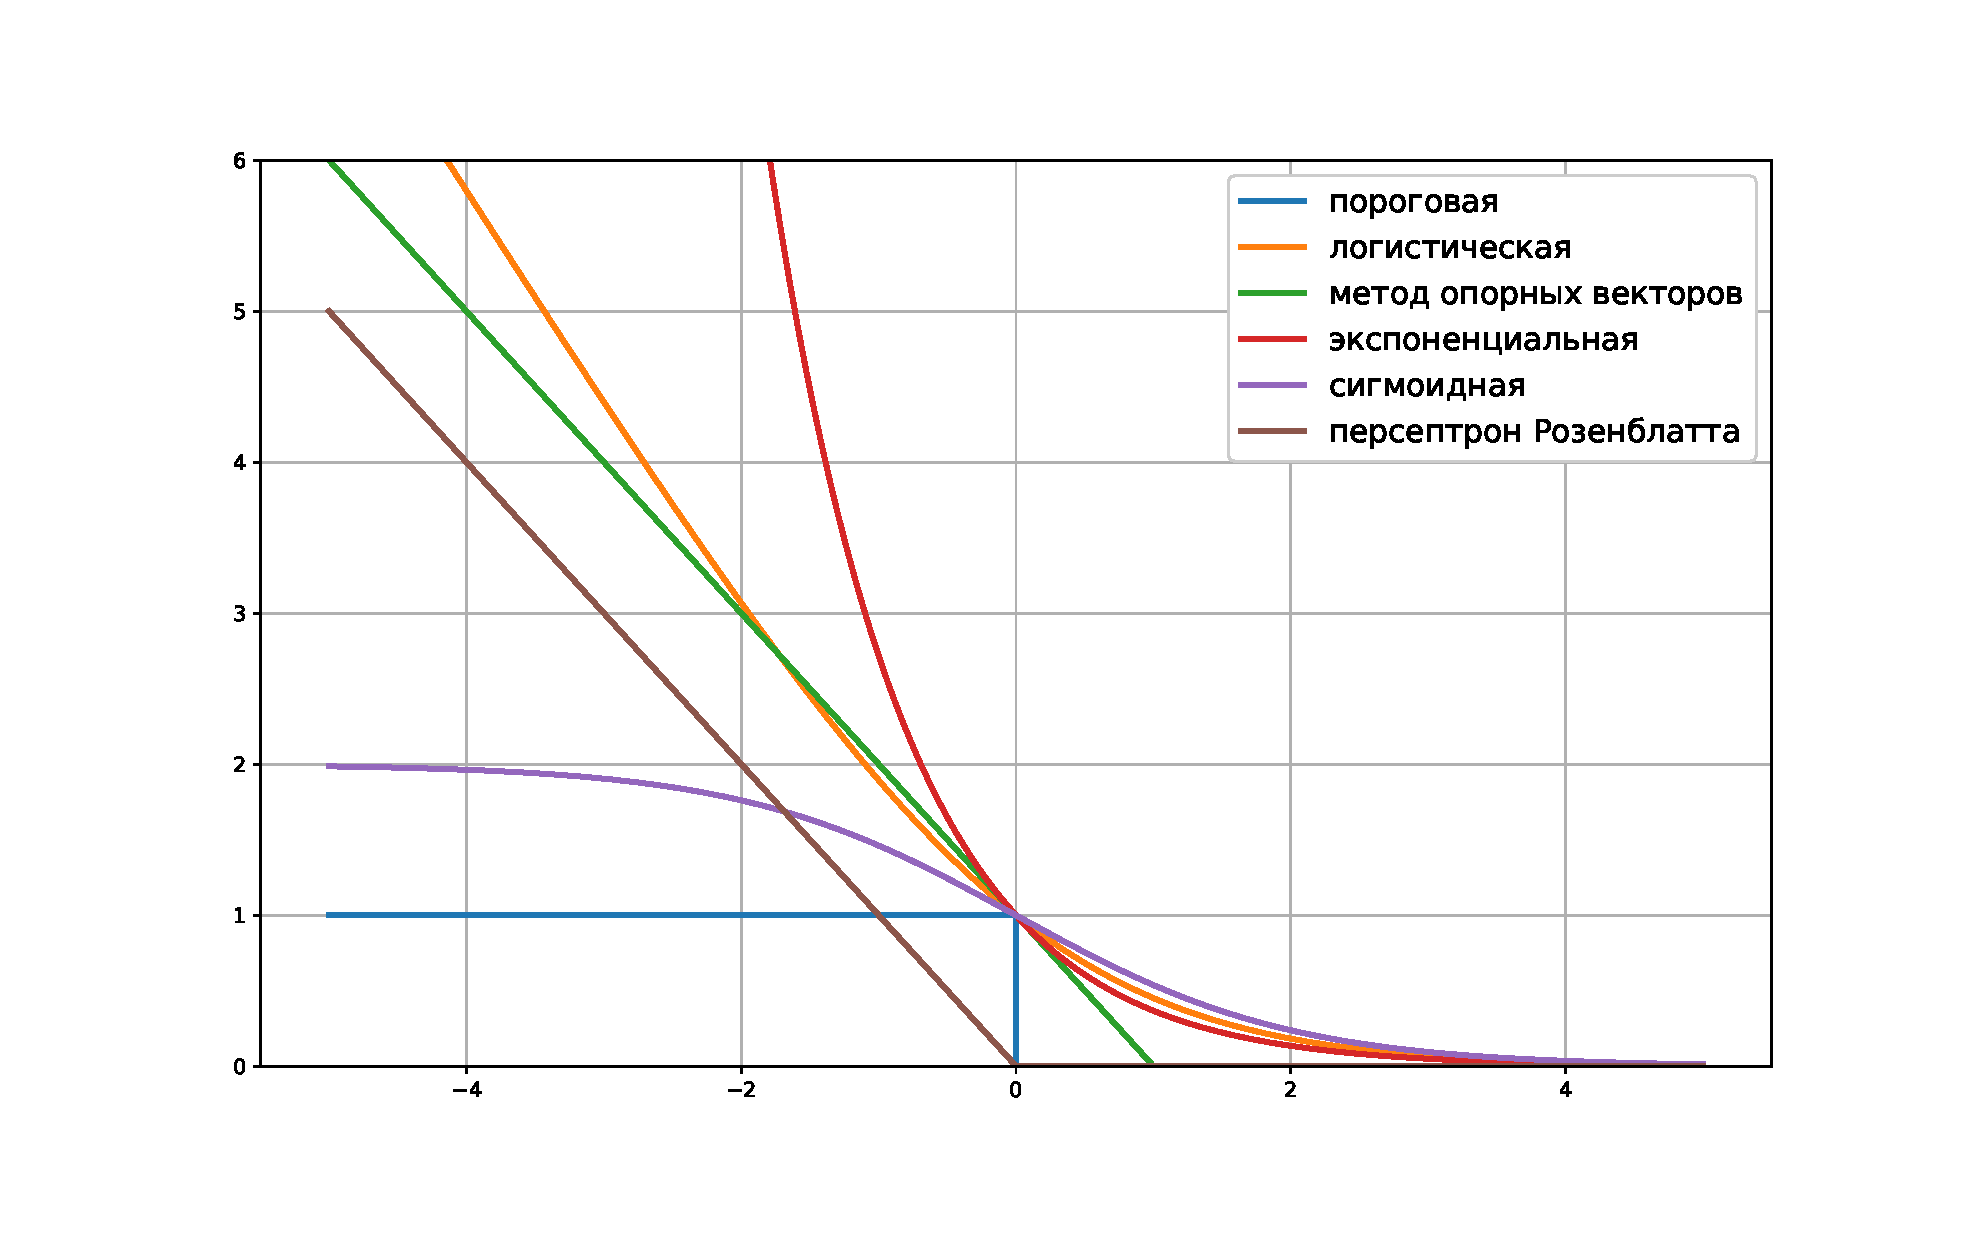
\includegraphics[width=0.8\textwidth]{threshold-approx.eps}
    \caption{Верхние оценки на пороговую функцию потерь.}
    \label{fig:bounds}
\end{figure}

Приведём несколько примеров верхних оценок:
\begin{enumerate}
    \item $\tilde L(M) = \log \left(1 + e^{-M} \right)$~--- логистическая функция потерь
    \item $\tilde L(M) = (1 - M)_+ = \max(0, 1 - M)$~--- кусочно-линейная функция потерь~(используется в методе опорных векторов)
    \item $\tilde L(M) = (-M)_+ = \max(0, -M)$~--- кусочно-линейная функция потерь~(соответствует персептрону Розенблатта)
    \item $\tilde L(M) = e^{-M}$~--- экспоненциальная функция потерь
    \item $\tilde L(M) = 2/(1 + e^M)$~--- сигмоидная функция потерь
\end{enumerate}
Любая из них подойдёт для обучения линейного классификатора.
Позже мы подробно изучим некоторые из них и выясним, какими свойствами они обладают.

\section{Метрики качества классификации}
Выше мы разобрали способ сведения задачи обучения линейного классификатора
к минимизации гладкого функционала.
При этом часто возникает необходимость в изучении различных аспектов качества
уже обученного классификатора.
Обсудим подробнее распространённые подходы к измерению качества таких моделей.

Будем считать, что классификатор имеет вид $a(x) = \sign(b(x) - t) = 2 [b(x) > t] - 1$.
Линейная модель имеет именно такую форму, если положить~$b(x) = \langle w, x \rangle$ и~$t = 0$.

\subsection{Доля правильных ответов}
Наиболее очевидной мерой качества в задаче классификации является доля правильных ответов~(accuracy),
которую мы уже упоминали:
\[
    \text{accuracy}(a, x)
    =
    \frac{1}{\ell}
    \sum_{i = 1}^{\ell} [a(x_i) = y_i].
\]
Данная метрика, однако, имеет существенный недостаток.
Если взять порог~$t$ меньше минимального значения прогноза~$b(x)$ на выборке
или больше максимального значения, то доля правильных ответов будет равна
доле положительных и отрицательных ответов соответственно.
Таким образом, если в выборке~$950$ отрицательных
и~$50$ положительных объектов, то при тривиальном пороге~$t = \max_i b(x_i)$
мы получим долю правильных ответов~$0.95$.
Это означает, что доля положительных ответов сама по себе
не несет никакой информации о качестве работы алгоритма~$a(x)$,
и вместе с ней следует анализировать соотношение классов в выборке.
Также полезно вместе с долей правильных ответов вычислять~\emph{базовую долю}~---
долю правильных ответов алгоритма, всегда выдающего наиболее мощный класс.

Отметим, что при сравнении различных методов машинного обучения
принято сообщать относительное уменьшение ошибки.
Рассмотрим два алгоритма~$a_1$ и~$a_2$ с долями правильных ответов~$r_1$ и~$r_2$
соответственно, причем~$r_2 > r_1$.
Относительным уменьшением ошибки алгоритма~$a_2$ называется величина
\[
    \frac{
        (1 - r_1) - (1 - r_2)
    }{
        1 - r_1
    }.
\]
Если доля ошибок была улучшена с~$20\%$ до~$10\%$,
то относительное улучшение составляет~$50\%$.
Если доля ошибок была улучшена с~$50\%$ до~$25\%$,
то относительное улучшение также равно~$50\%$,
хотя данный прирост кажется более существенным.
Если же доля ошибок была улучшена с~$0.1\%$ до~$0.01\%$,
то относительное улучшение составляет~$90\%$,
что совершенно не соответствует здравому смыслу.

\subsection{Матрица ошибок}
Выше мы убедились, что в случае с несбалансированными классами
одной доли правильных ответов недостаточно~--- необходима еще
одна метрика качества.
В данном разделе мы рассмотрим другую, более информативную пару критериев.

Введем сначала понятие матрицы ошибок.
Это способ разбить объекты на четыре категории в зависимости
от комбинации истинного ответа и ответа алгоритма~(см. таблицу~\ref{tbl:confusion}).
Через элементы этой матрицы можно, например, выразить долю правильных ответов:
\[
    \text{accuracy}
    =
    \frac{\text{TP} + \text{TN}}{\text{TP} + \text{FP} + \text{FN} + \text{TN}}.
\]

Гораздо более информативными критериями являются~\emph{точность}~(precision)
и~\emph{полнота}~(recall):
\begin{align*}
    &\text{precision}
    =
    \frac{
        \text{TP}
    }{
        \text{TP} + \text{FP}
    };\\
    &\text{recall}
    =
    \frac{
        \text{TP}
    }{
        \text{TP} + \text{FN}
    }.
\end{align*}
Точность показывает, какая доля объектов, выделенных классификатором как положительные,
действительно является положительными.
Полнота показывает, какая часть положительных объектов была выделена классификатором.

\begin{table}[t]
    \centering
    \begin{tabular}{|c|c|c|}
        \hline
        & $y = 1$ & $y = -1$ \\ \hline
        $a(x) = 1$ & True Positive (TP) & False Positive (FP) \\ \hline
        $a(x) = -1$ & False negative (FN) & True Negative (TN) \\ \hline
    \end{tabular}
    \caption{Матрица ошибок}
    \label{tbl:confusion}
\end{table}

Рассмотрим, например, задачу предсказания реакции клиента банка на звонок с предложением кредита.
Ответ~$y = 1$ означает, что клиент возьмет кредит после рекламного звонка,
ответ~$y = -1$~--- что не возьмет.
Соответственно, планируется обзванивать только тех клиентов, для которых
классификатор~$a(x)$ вернет ответ~$1$.
Если классификатор имеет высокую точность, то практически все клиенты, которым
будет сделано предложение, откликнутся на него.
Если классификатор имеет высокую полноту, то предложение будет сделано практически
всем клиентам, которые готовы откликнуться на него.
Как правило, можно регулировать точность и полноту, изменяя порог~$t$
в классификаторе~$a(x) = \sign(b(x) - t) = 2 [b(x) > t] - 1$.
Если выбрать~$t$ большим, то классификатор будет относить к положительному классу
небольшое число объектов, что приведет к высокой точности и низкой полноте.
По мере уменьшения~$t$ точность будет падать, а полнота увеличиваться.
Конкретное значение порога выбирается согласно пожеланиям заказчика.

Отметим, что точность и полнота не зависят от соотношения размеров классов.
Даже если объектов положительного класса на порядки меньше,
чем объектов отрицательного класса, данные показатели будут корректно
отражать качество работы алгоритма.

Существует несколько способов получить один критерий качества
на основе точности и полноты.
Один из них~--- F-мера, гармоническое среднее точности и полноты:
\[
    F
    =
    \frac{
        2 * \text{precision} * \text{recall}
    }{
        \text{precision} + \text{recall}
    }.
\]
Среднее гармоническое обладает важным свойством~--- оно близко к нулю, если хотя бы
один из аргументов близок к нулю.
Именно поэтому оно является более предпочтительным, чем среднее арифметическое~(если
алгоритм будет относить все объекты к положительному классу,
то он будет иметь~$\text{recall} = 1$ и~$\text{precision} \ll 1$,
а их среднее арифметическое будет больше~$1/2$, что недопустимо).
Можно заметить, что F-мера является сглаженной версией минимума
из точности и полноты~(см. рис.~\ref{fig:curvesMin} и~\ref{fig:curvesHarmonic}).
Отметим, что геометрическое среднее также похоже на сглаженный вариант минимума,
но при этом оно менее устойчиво к~<<выбросам>>~--- например, для точности~0.9
и полноты~0.1 гармоническое среднее будет равно~0.18, а геометрическое~0.3.

\begin{figure}[t]
  \begin{multicols}{2}
    \hfill
    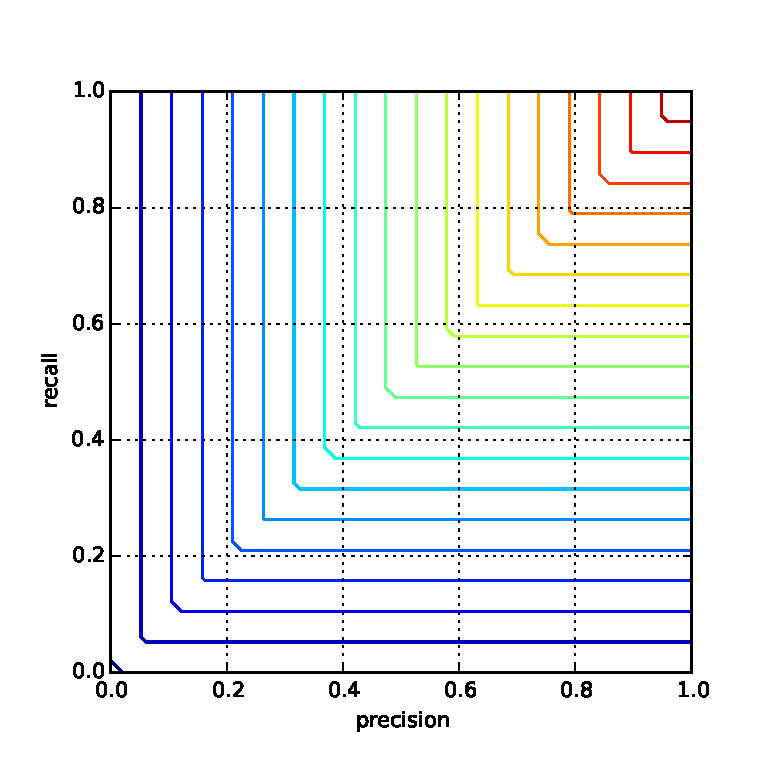
\includegraphics[width=70mm]{precision_recall_min.eps}
    \hfill
    \caption{Линии уровня для минимума из точности и полноты.}
    \label{fig:curvesMin}
    \hfill
    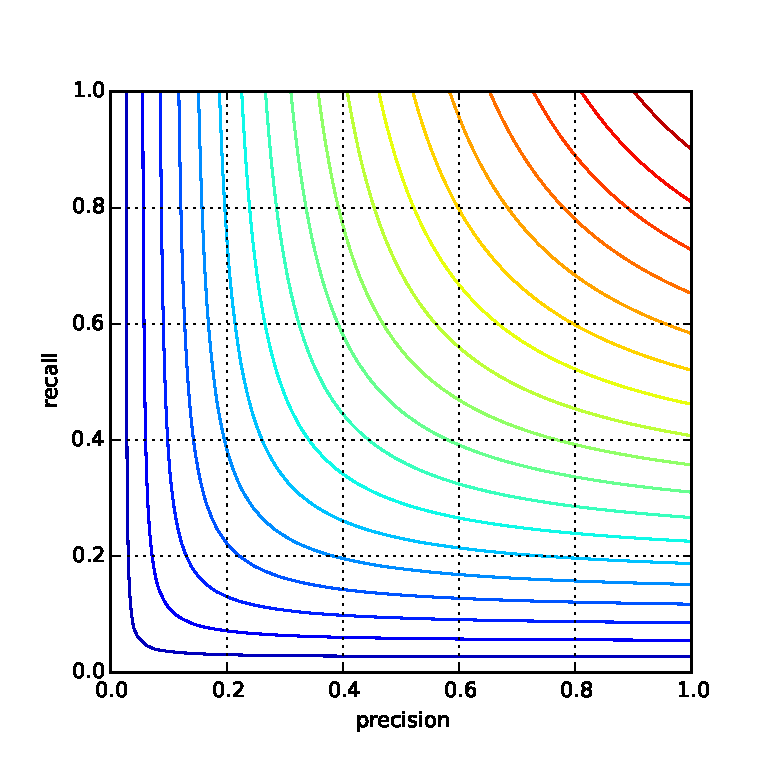
\includegraphics[width=70mm]{precision_recall_harmonic.eps}
    \hfill
    \caption{Линии уровня для F-меры.}
    \label{fig:curvesHarmonic}
  \end{multicols}
\end{figure}

Другим агрегированным критерием является~\emph{R-точность},
или точка баланса~(breakeven point).
Она вычисляется как точность при таком~$t$, при котором полнота равна точности:
\begin{align*}
    &\text{R-precision}
    =
    \text{precision}(\sign(b(x) - t^*)),\\
    &t^* = \argmin_t \left|
        \text{precision}(\sign(b(x) - t))
        -
        \text{recall}(\sign(b(x) - t))
    \right|.
\end{align*}
Можно показать, что R-точность равна точности при таком пороге,
при котором количество отнесённых к положительному классу объектов
равно количеству положительных объектов в выборке.

Часто встречаются задачи, в которых целевой признак по-прежнему бинарный,
но при этом необходимо ранжировать объекты, а не просто предсказывать их класс.
Например, в задаче предсказания реакции клиента можно выдавать сортированный список,
чтобы оператор мог в первую очередь позвонить клиентам с наибольшей вероятностью
положительного отклика.
Поскольку многие алгоритмы возвращают вещественный ответ~$b(x)$,
который затем бинаризуется по порогу~$t$,
то можно просто сортировать объекты по значению~$b(x)$.
Для измерения качества ранжирования нередко используют~\emph{среднюю точность}~(average precision, AP):
\[
    \text{AP}
    =
    \frac{1}{\ell_{+}}
    \sum_{k = 1}^{\ell}
        [y_{(k)} = 1] \text{precision}@k,
\]
где~$y_{(k)}$~--- ответ~$k$-го по порядку объекта,
$\ell_{+}$~--- число положительных объектов в выборке,
а~$\text{precision}@k$~--- точность среди первых~$k$ в списке объектов.
Если алгоритм~$b(x)$ так ранжирует объекты, что сначала идут все положительные,
а затем все отрицательные, то средняя точность будет равна единице;
соответственно, чем сильнее положительные документы концентрируются в верхней
части списка, тем ближе к единице будет данный показатель.

\paragraph{Связь точности, полноты и доли правильных ответов}
Выше мы отмечали, что высокие значения доли правильных ответов вовсе не влекут
за собой высокое качество работы классификатора,
и ввели точность и полноту как способ решения этой проблемы.
Тем не менее, при выборе точности и полноты в качестве основных метрик, следует
соблюдать осторожность при выборе требований к их значениям~--- как мы увидим из примера,
независимость данных метрик от соотношения классов может привести к неочевидным последствиям.

Рассмотрим задачу бинарной классификации с миллионом объектов~($\ell = 1.000.000$),
где доля объектов первого класса составляет $1\%$~($\ell_+ = 10.000$).
Мы знаем, что доля правильных ответов будет вести себя не вполне интуитивно
на данной несбалансированной выборке, и поэтому выберем точность и полноту для измерения
качества классификаторов.
Поскольку мы хотим решить задачу хорошо, то введём требования, что и точность, и полнота
должны быть не менее~$90\%$.
Эти требования кажутся вполне разумными, если забыть о соотношении классов.
Попробуем теперь оценить, какая доля правильных ответов должна быть у классификатора,
удовлетворяющего нашим требованиям.

Всего в выборке~$10.000$ положительных объектов, и для достижения полноты~$90\%$
мы должны отнести как минимум~$9.000$ к положительному классу.
Получаем~$\text{TP} = 9000$, $\text{FN} = 1000$.
Так как точность тоже должна быть не меньше~$90\%$, получаем~$\text{FP} = 1000$.
Отсюда получаем, что доля правильных ответов должна быть равна~$(1 - 2.000/1.000.000) = 99.8\%$!
Это крайне высокий показатель, и его редко удаётся достичь на таких выборках во многих предметных областях.

\paragraph{Lift.}
На практике часто возникают задачи, связанные с выбором подмножества: выделение лояльных клиентов банка,
обнаружение уходящих пользователей мобильного оператора и т.д.
Заказчика может интересовать вопрос, насколько выгоднее работать с этим подмножеством
по сравнению со всем множеством.
Если при рассылке предложений о кредите клиентам из подмножества и всем клиентам
будет получаться одна и та же доля откликнувшихся, то подмножество не будет
представлять особой ценности.
Формально это измеряется с помощью~\emph{прироста концентрации}~(lift),
который равен отношению точности к доле положительных объектов в выборке:
\[
    \text{lift}
    =
    \frac{
        \text{precision}
    }{
        (\text{TP} + \text{FN}) / \ell
    }.
\]
Эту величину можно интерпретировать как улучшение доли положительных объектов
в данном подмножестве относительно доли в случайно выбранном подмножестве такого же размера.

\subsection{Area Under Curve}
Выше мы изучили точность, полноту и F-меру, которые характеризуют
качество работы алгоритма~$a(x) = \sign(b(x) - t)$ при конкретном выборе порога~$t$.
Однако зачастую интерес представляет лишь вещественнозначный алгоритм~$b(x)$,
а порог будет выбираться позже в зависимости от требований к точности и полноте.
В таком случае возникает потребность
в измерении качества семейства моделей~$\{a(x) = \sign(b(x) - t) \cond t \in \RR\}$.

\begin{figure}[t]
    \centering
    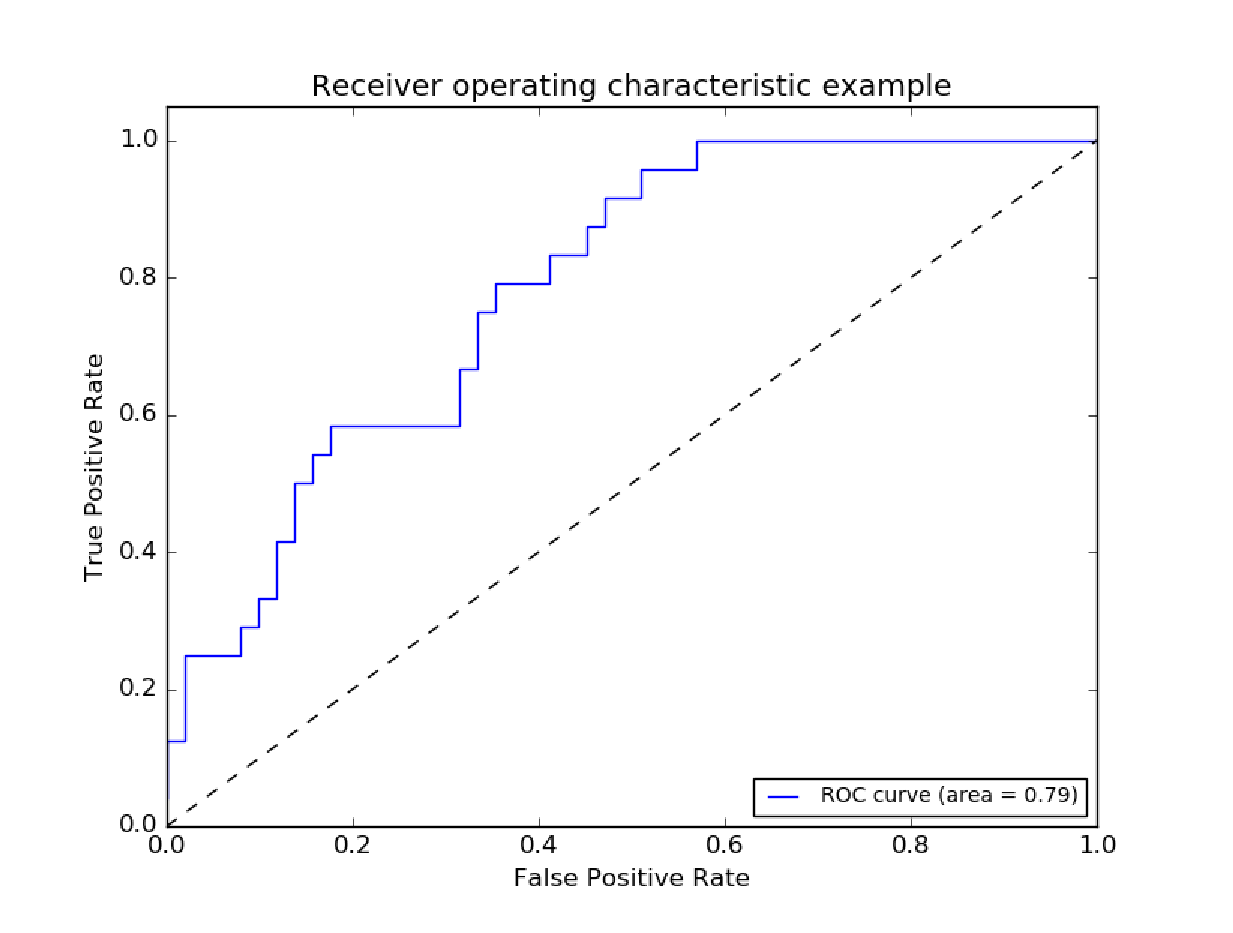
\includegraphics[width=0.7\textwidth]{plot_roc_001.eps}
    \caption{Пример ROC-кривой.}
    \label{fig:roc}
\end{figure}

Можно измерять качество этого множества на основе качества лучшего~(в некотором смысле) алгоритма.
Для этого подходит упомянутая ранее точка баланса~(breakeven point).
В идеальном семействе алгоритмов она будет равна единице, поскольку найдется
алгоритм со стопроцентной точностью и полнотой.
Данная метрика, однако, основывается лишь на качестве одного алгоритма,
и не характеризует вариативность семейства.

Широко используется такая интегральная метрика качества семейства,
как~\emph{площадь под ROC-кривой}~(Area Under ROC Curve, AUC-ROC).
Рассмотрим двумерное пространство, одна из координат которого соответствует
доле неверно принятых объектов~(False Positive Rate, FPR),
а другая~--- доле верно принятых объектов~(True Positive Rate, TPR):
\begin{align*}
    &\text{FPR}
    =
    \frac{
        \text{FP}
    }{
        \text{FP} + \text{TN}
    };\\
    &\text{TPR}
    =
    \frac{
        \text{TP}
    }{
        \text{TP} + \text{FN}
    }.
\end{align*}
Каждый возможный выбор порога~$t$ соответствует точке в этом пространстве.
Всего различных порогов имеется~$\ell + 1$.
Максимальный порог~$t_{\max} = \max_{i} b(x_i)$ даст классификатор
с~$\text{TPR} = 0$, $\text{FPR} = 0$.
Минимальный порог~$t_{\min} = \min_{i} b(x_i) - \eps$ даст~$\text{TPR} = 1$
и~$\text{FPR} = 1$.
ROC-кривая~--- это кривая с концами в точках~$(0, 0)$ и~$(1, 1)$,
которая последовательно соединяет точки, соответствующие
порогам~$b(x_{(1)}) - \eps, b(x_{(1)}), b(x_{(2)}), \dots, b(x_{(\ell)})$~(см. рис.~\ref{fig:roc}).
Площадь под данной кривой называется AUC-ROC, и принимает значения от~$0$ до~$1$.
Если порог~$t$ может быть подобран так, что алгоритм~$a(x)$ не будет допускать ошибок,
то AUC-ROC будет равен единице;
если же~$b(x)$ ранжирует объекты случайным образом, то AUC-ROC будет близок к~$0.5$.

Критерий AUC-ROC имеет большое число интерпретаций~--- например,
он равен вероятности того, что для случайно выбранных
положительного объекта~$x_+$ и отрицательного объекта~$x_-$
будет выполнено\footnote{При условии, что прогнозы на всех объектах выборки попарно различны.}~$b(x_+) > b(x_-)$.

%Разберем подробнее немного другую формулировку.

%\begin{vkProblem}
%    В ранжировании часто используется функционал~<<доля дефектных пар>>.
%    Его можно определить и для задачи бинарной классификации.

%    Пусть дан классификатор~$b(x)$, который возвращает оценки принадлежности объектов
%    классам: чем больше ответ классификатора, тем более он уверен в том, что данный объект
%    относится к классу~<<$+1$>>.
%    Отсортируем все объекты по неубыванию ответа классификатора~$b$:~$x_{(1)}, \dots, x_{(\ell)}$.
%    Обозначим истинные ответы на этих объектах через~$y_{(1)}, \dots, y_{(\ell)}$.
%    Тогда доля дефектных пар записывается как
%    \[
%        \text{DP}(a, X^\ell)
%        =
%        \frac{2}{\ell (\ell - 1)}
%        \sum_{i < j}^{\ell}
%            \left[
%                y_{(i)} > y_{(j)}
%            \right].
%    \]

%    Как данный функционал связан с AUC-ROC?
%\end{vkProblem}

%\begin{esSolution}
%    Разберем процедуру построения AUC-ROC.
%    Сначала все объекты сортируются по оценке классификатора.
%    Стартуем из точки~$(0, 0)$~--- она соответствует порогу~$y_{(\ell)}$.
%    Начинаем идти от большей оценки к меньшей.
%    Если текущий объект имеет класс~<<$1$>>, то у алгоритма увеличивается~TPR;
%    значит, ROC-кривая сдвигается вверх на~$1 / \ell_{+}$~($\ell_{+}$~--- число объектов положительного класса).
%    Если у текущего объекта класс <<$0$>>, то алгоритм допускает на одну ошибку больше,
%    чем предыдущий~--- значит, ROC-кривая сдвигается вправо
%    на~$1 / \ell_{-}$~($\ell_{-}$~--- число объектов отрицательного класса),
%    а к AUC надо прибавить~$\sum_{j = i + 1}^{\ell} [y_{(j)} = +1] / (\ell_{+} \ell_{-})$.
%    Получаем:
%    \begin{align*}
%        \text{AUC}
%        =
%        \frac{1}{\ell_{+} \ell_{-}}
%        &\sum_{i = 1}^{\ell}
%            [y_{(i)} = 0]
%            \sum_{j = i + 1}^{\ell}
%                [y_{(j)} = +1]
%        =\\
%        &=
%        \frac{1}{\ell_{+} \ell_{-}}
%        \sum_{i = 1}^{\ell} \sum_{j = i + 1}^{\ell}
%            [y_{(i)} < y_{(j)}]
%        =\\
%        &=
%        \frac{1}{\ell_{+} \ell_{-}}
%        \sum_{i < j}^{\ell}
%            (1 - [y_{(i)} > y_{(j)}] - [y_{(j)} = y_{(i)}])
%        =\\
%        &=
%        \frac{1}{\ell_{+} \ell_{-}}
%        \sum_{i < j}^{\ell}
%            (1 - [y_{(j)} = y_{(i)}])
%        -
%        \frac{1}{\ell_{+} \ell_{-}}
%        \sum_{i < j}^{\ell}
%            [y_{(i)} > y_{(j)}]
%        =\\
%        &=
%        \frac{1}{\ell_{+} \ell_{-}}
%        \frac{\ell (\ell - 1)}{2}
%        -
%        \frac{\ell_+ (\ell_+ - 1)}{2 \ell_+ \ell_-}
%        -
%        \frac{\ell_- (\ell_- - 1)}{2 \ell_+ \ell_-}
%        -
%        \frac{1}{\ell_{+} \ell_{-}}
%        \sum_{i < j}^{\ell}
%            [y_{(i)} > y_{(j)}]
%        =\\
%        &=
%        1
%        -
%        \frac{1}{\ell_{+} \ell_{-}}
%        \sum_{i < j}
%            [y_{(i)} > y_{(j)}].
%    \end{align*}

%    Получаем, что AUC связан с числом дефектных пар~$\text{DP}$ формулой
%    \[
%        \text{DP}
%        =
%        \frac{2 \ell_{-} \ell_{+}}{\ell (\ell - 1)}
%        (1 - \text{AUC}).
%    \]
%\end{esSolution}

\paragraph{Индекс Джини.}
В задачах кредитного скоринга вместо AUC-ROC часто используется пропорциональная
метрика, называемая индексом Джини~(Gini index):
\[
    \text{Gini}
    =
    2 \text{AUC} - 1.
\]
По сути это умноженная на два площадь между ROC-кривой и диагональю, соединяющей точки~$(0, 0)$ и~$(1, 1)$.

Отметим, что переход от AUC к индексу Джини приводит к увеличению относительных разниц.
Если мы смогли улучшить AUC с~$0.8$ до~$0.9$, то это соответствует
относительному улучшению в~$12.5\%$.
В то же время соответствующие индексы Джини были улучшены с~$0.6$ до~$0.8$,
то есть на~$33.3\%$~--- относительное улучшение повысилось почти в три раза!

\paragraph{Чувствительность к соотношению классов.}
Рассмотрим задачу выделения математических статей из множества научных статей.
Допустим, что всего имеется~$1.000.100$ статей, из которых лишь~$100$ относятся к математике.
Если нам удастся построить алгоритм~$a(x)$, идеально решающий задачу,
то его~TPR будет равен единице, а~FPR~--- нулю.
Рассмотрим теперь плохой алгоритм, дающий положительный ответ на~$95$ математических
и~$50.000$ нематематических статьях.
Такой алгоритм совершенно бесполезен, но при этом имеет~$\text{TPR} = 0.95$
и~$\text{FPR} = 0.05$, что крайне близко к показателям идеального алгоритма.

Таким образом, если положительный класс существенно меньше по размеру,
то AUC-ROC может давать неадекватную оценку качества работы алгоритма,
поскольку измеряет долю неверно принятых объектов относительно
общего числа отрицательных.
Так, алгоритм~$b(x)$, помещающий~$100$ релевантных документов
на позиции с~$50.001$-й по~$50.101$-ю, будет иметь AUC-ROC~$0.95$.

\paragraph{Precison-recall кривая.}
Избавиться от указанной проблемы с несбалансированными классами можно,
перейдя от ROC-кривой к Precision-Recall кривой.
Она определяется аналогично ROC-кривой, только по осям
откладываются не FPR и TPR, а полнота~(по оси абсцисс) и точность~(по оси ординат).
Критерием качества семейства алгоритмов выступает площадь под PR-кривой~(AUC-PR).
Данную величину можно аппроксимировать следующим образом.
Стартуем из точки~$(0, 1)$.
Будем идти по ранжированной выборке, начиная с первого объекта;
пусть текущий объект находится на позиции~$k$.
Если он относится к классу~<<$-1$>>,
то полнота не меняется, точность падает~--- соответственно, кривая опускается строго вниз.
Если же объект относится к классу~<<$1$>>,
то полнота увеличивается на~$1/\ell_{+}$, точность растет, и кривая поднимается вправо и вверх.
Площадь под этим участком можно аппроксимировать площадью прямоугольника
с высотой, равной~$\text{precision}@k$ и шириной~$1/\ell_{+}$.
При таком способе подсчета площадь под PR-кривой будет совпадать со средней точностью:
\[
    \text{AUC-PR}
    =
    \frac{1}{\ell_{+}}
    \sum_{k = 1}^{\ell}
        [y_k = 1]
        \text{precision}@k.
\]

Отметим, что AUC-PR дает разумные результаты в рассмотренном выше примере с классификацией статей.
Так, при размещении~$100$ релевантных документов на позициях~$50.001$-$50.101$ в ранжированном списке,
AUC-PR будет равен~0.001.

Несмотря на указанные различия, между ROC- и PR-кривой имеется тесная связь.
Так, можно показать, что если ROC-кривая одного алгоритма лежит полностью над
ROC-кривой другого алгоритма, то и PR-кривая одного лежит над PR-кривой другого~\cite{davis06pr}.

\begin{thebibliography}{1}
\bibitem{davis06pr}
    \emph{Davis J., Goadrich M.} (2006).
    The Relationship Between Precision-Recall and ROC Curves.~//
    Proceedings of the 23rd International Conference on Machine Learning, Pittsburgh, PA.
\end{thebibliography}

\end{document}
